\begin{figure*}[!htb]
\centering
  \vspace{-1.7cm}
  \begin{tabular}{cccc}
    % \raisebox{4.5cm}
    \raisebox{3.8cm}{\panel{A}} &
    {\hspace{-0.cm}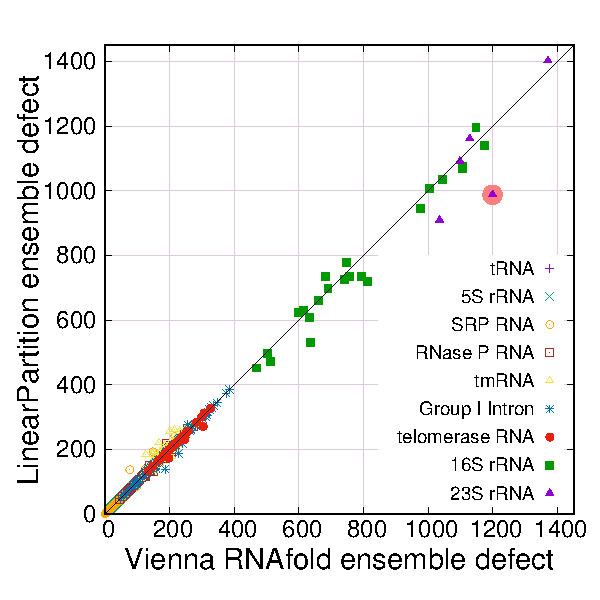
\includegraphics[width=0.24\textwidth]{figs/ensemble_defect}} &
    \raisebox{3.8cm}{\hspace{1.4cm}\panel{B}} &
    \raisebox{-0.3cm}{\hspace{-1.2cm}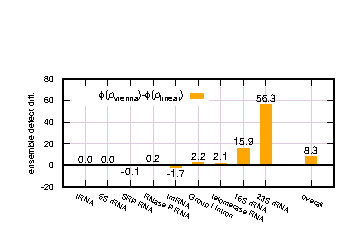
\includegraphics[width=0.5\textwidth]{figs/ensemble_defect_histogram}}
  \end{tabular}
  \\[-0.4cm]
%   \vspace{-.5cm}
  \begin{tabular}{ccccc}
&\hspace{-4.cm} \panel{C} & \hspace{-4.6cm}\panel{D} & \hspace{-4.6cm}\panel{E} & \hspace{-4.6cm}\panel{F}\\[-0.3cm]
\raisebox{.9cm}{\rotatebox{90}{\ecoli 23S rRNA}}&
\hspace{-0.2cm}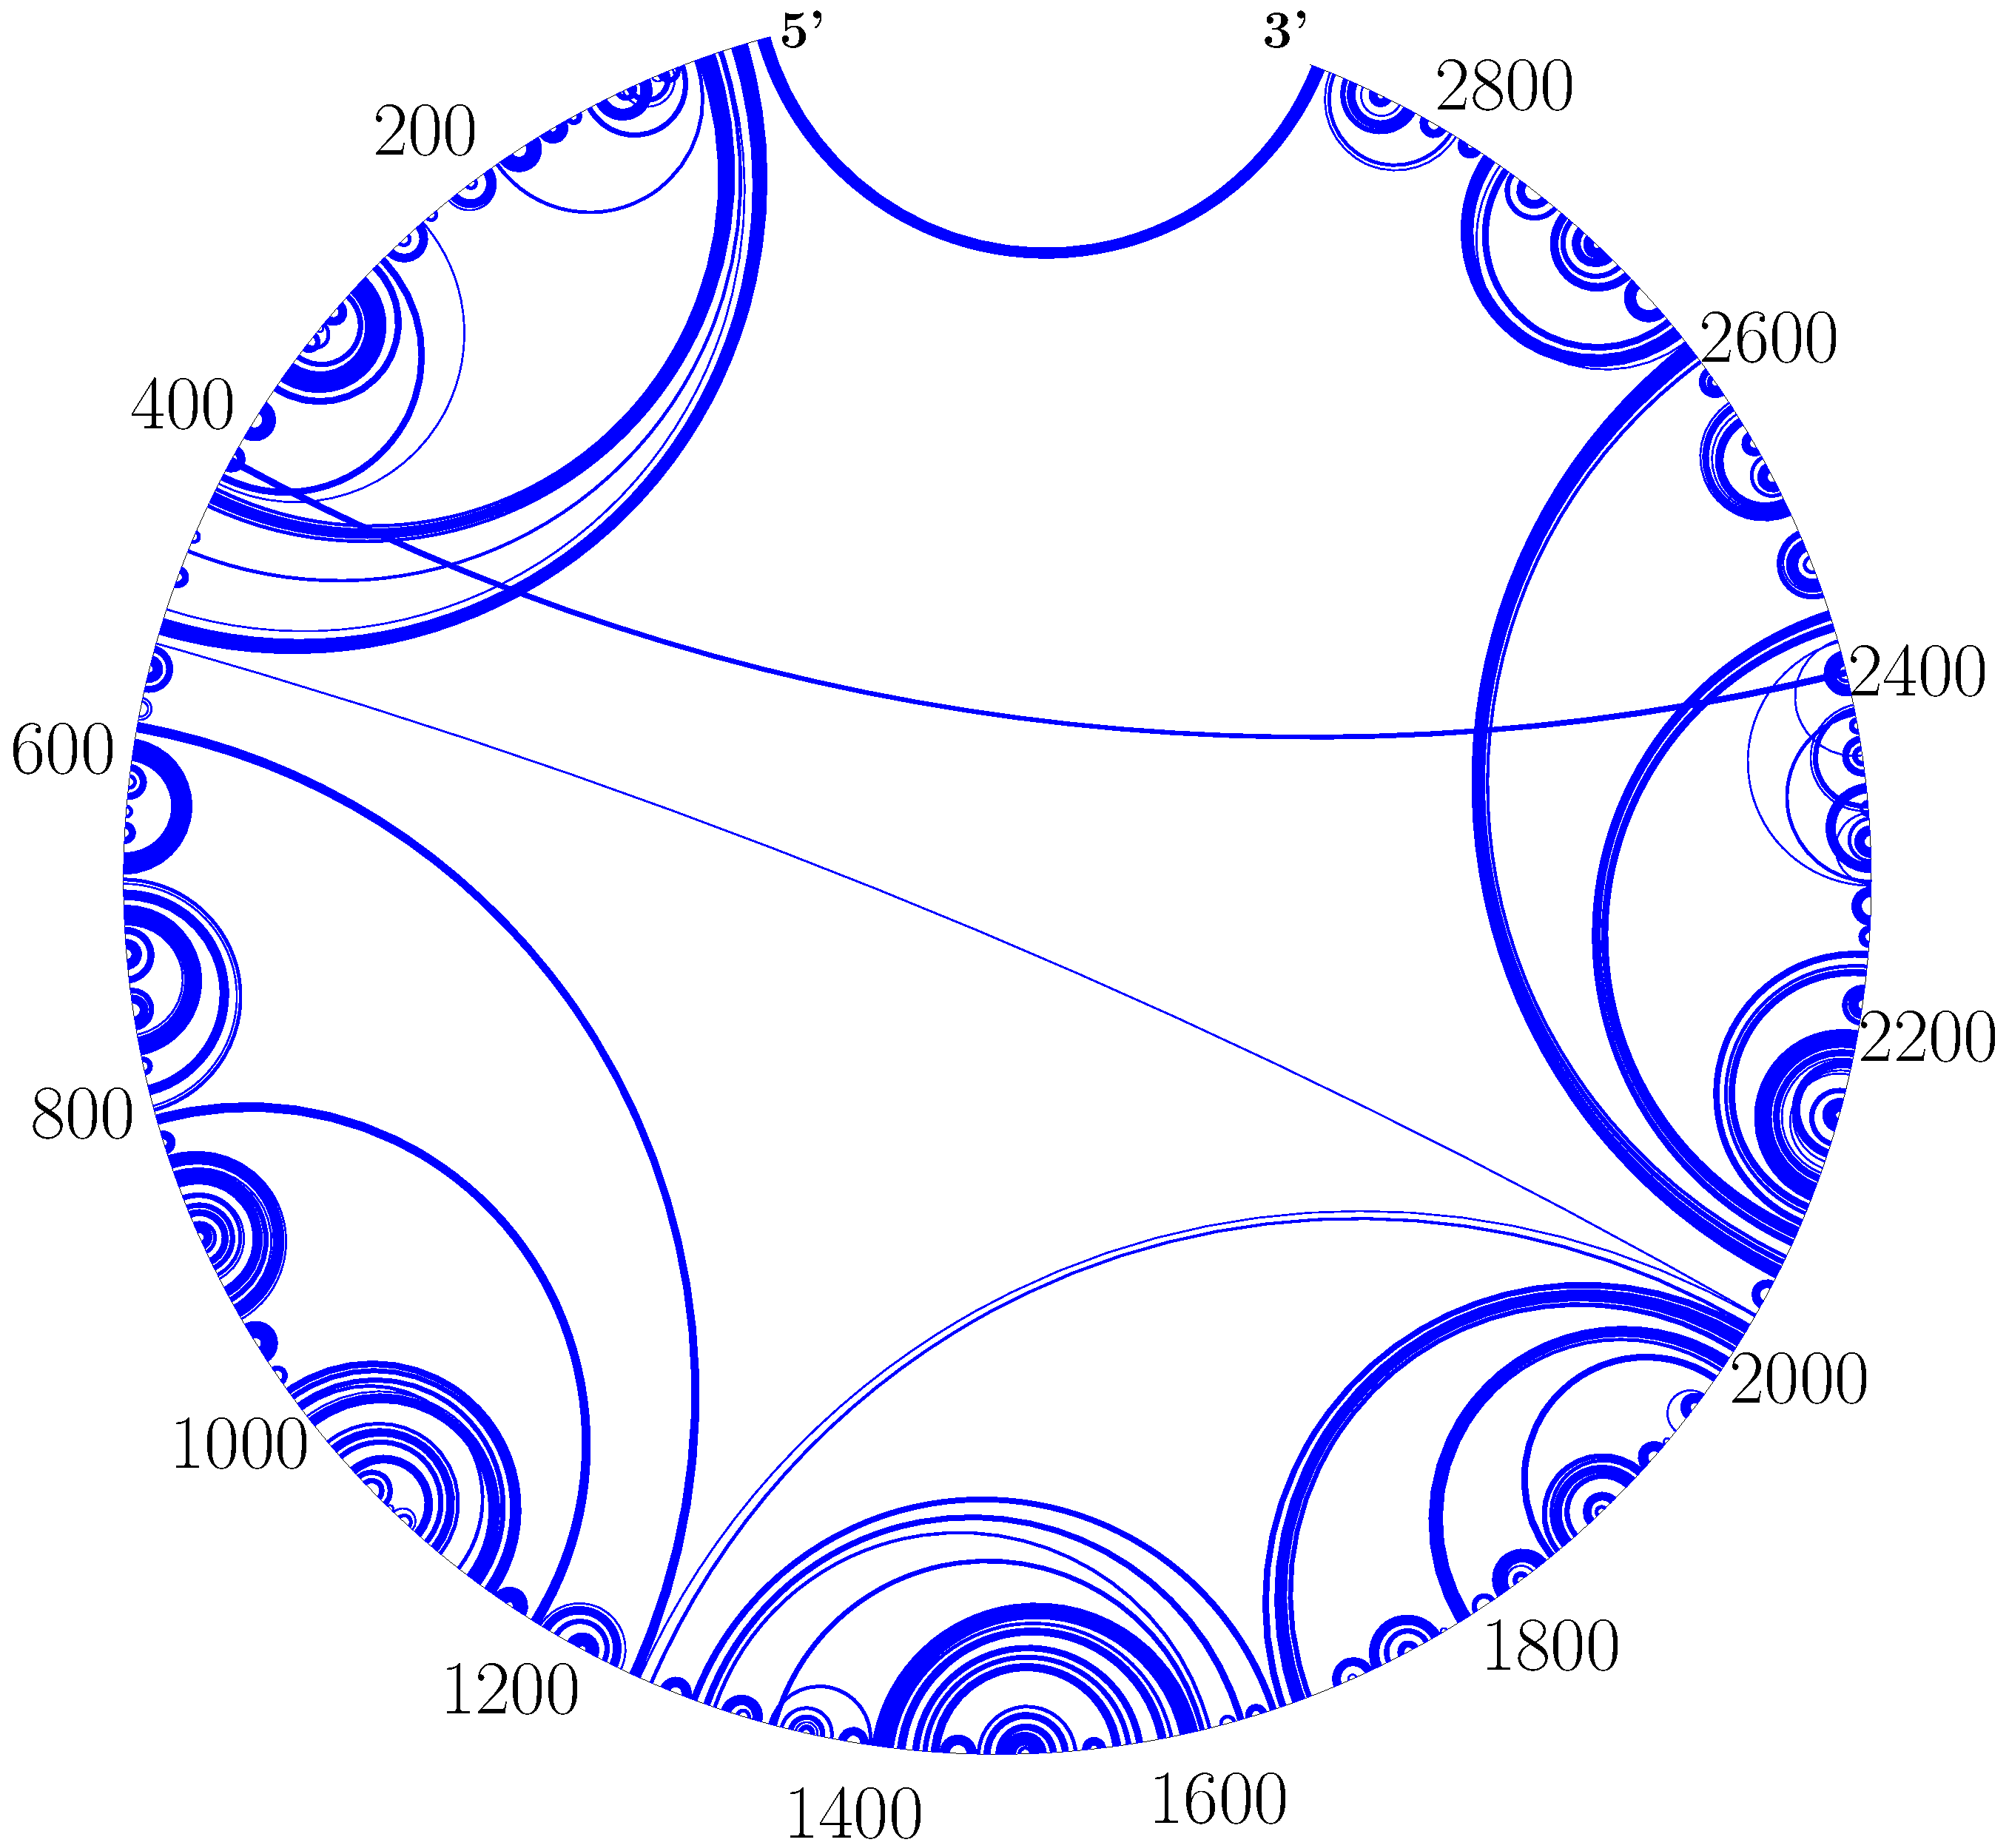
\includegraphics[width=0.22\textwidth]{figs/23s_gold} &
\hspace{-0.35cm}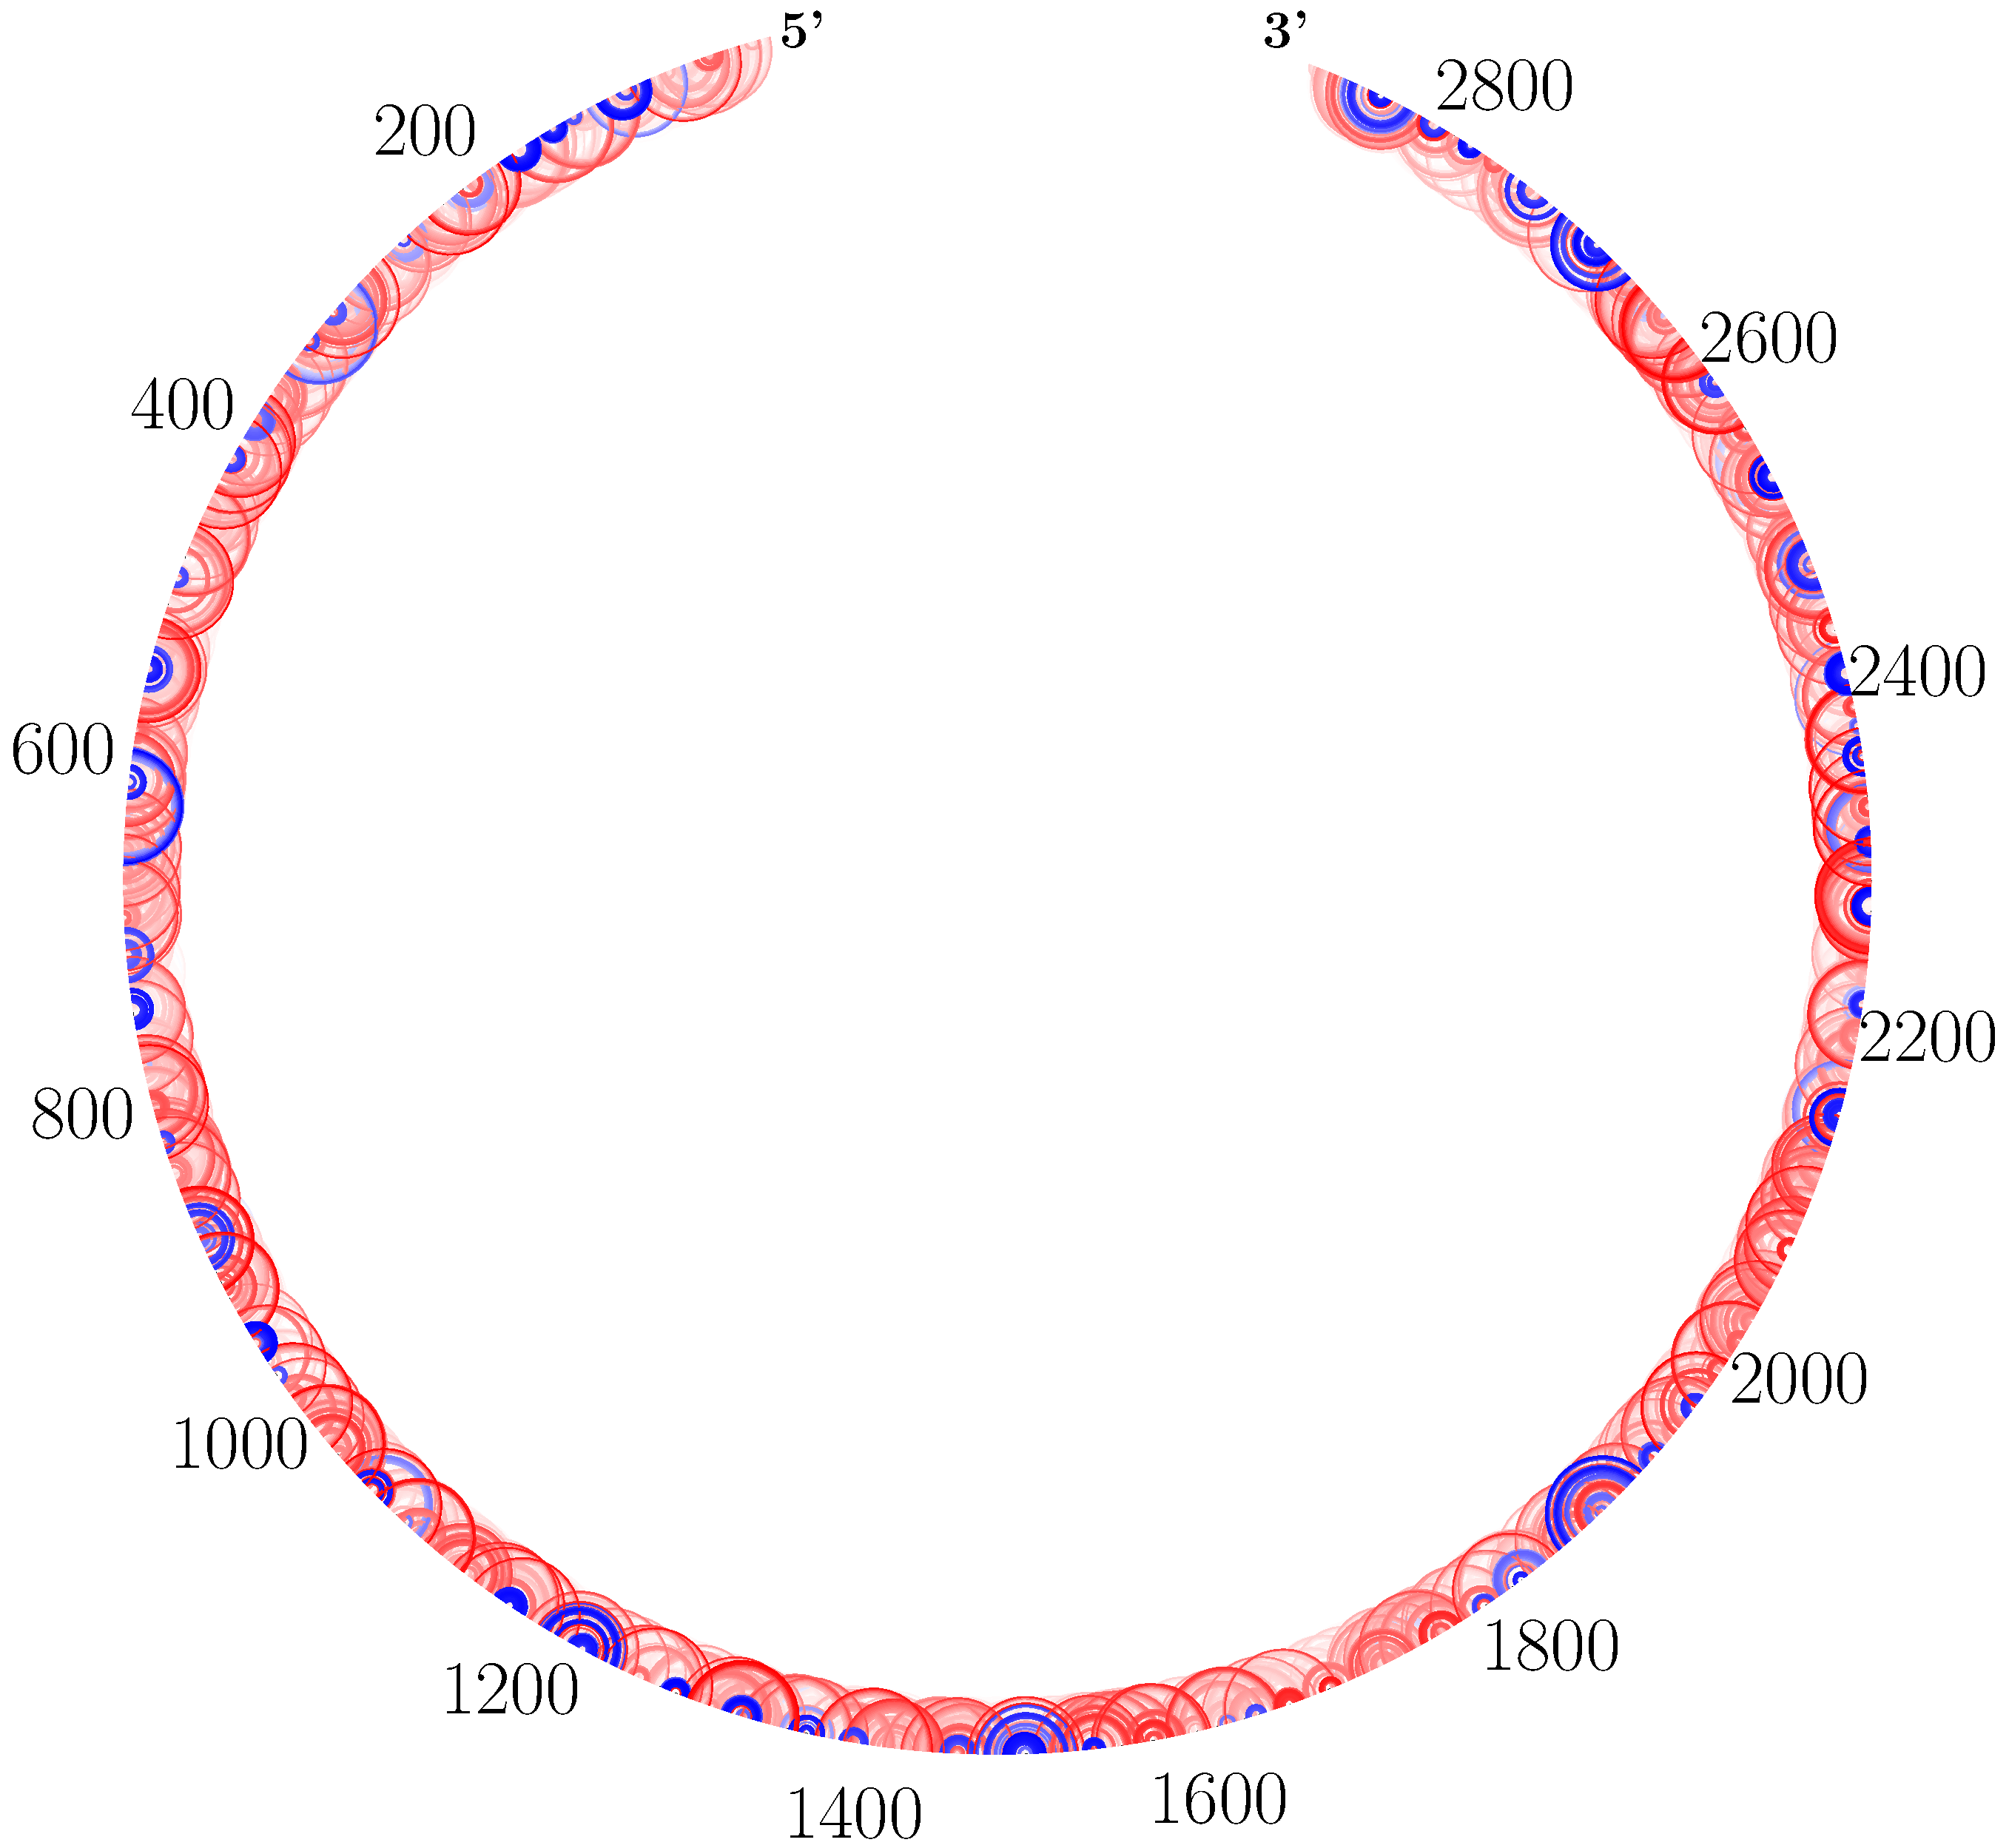
\includegraphics[width=0.22\textwidth]{figs/23s_vienna_plfold_example.pdf} &
\hspace{-0.35cm}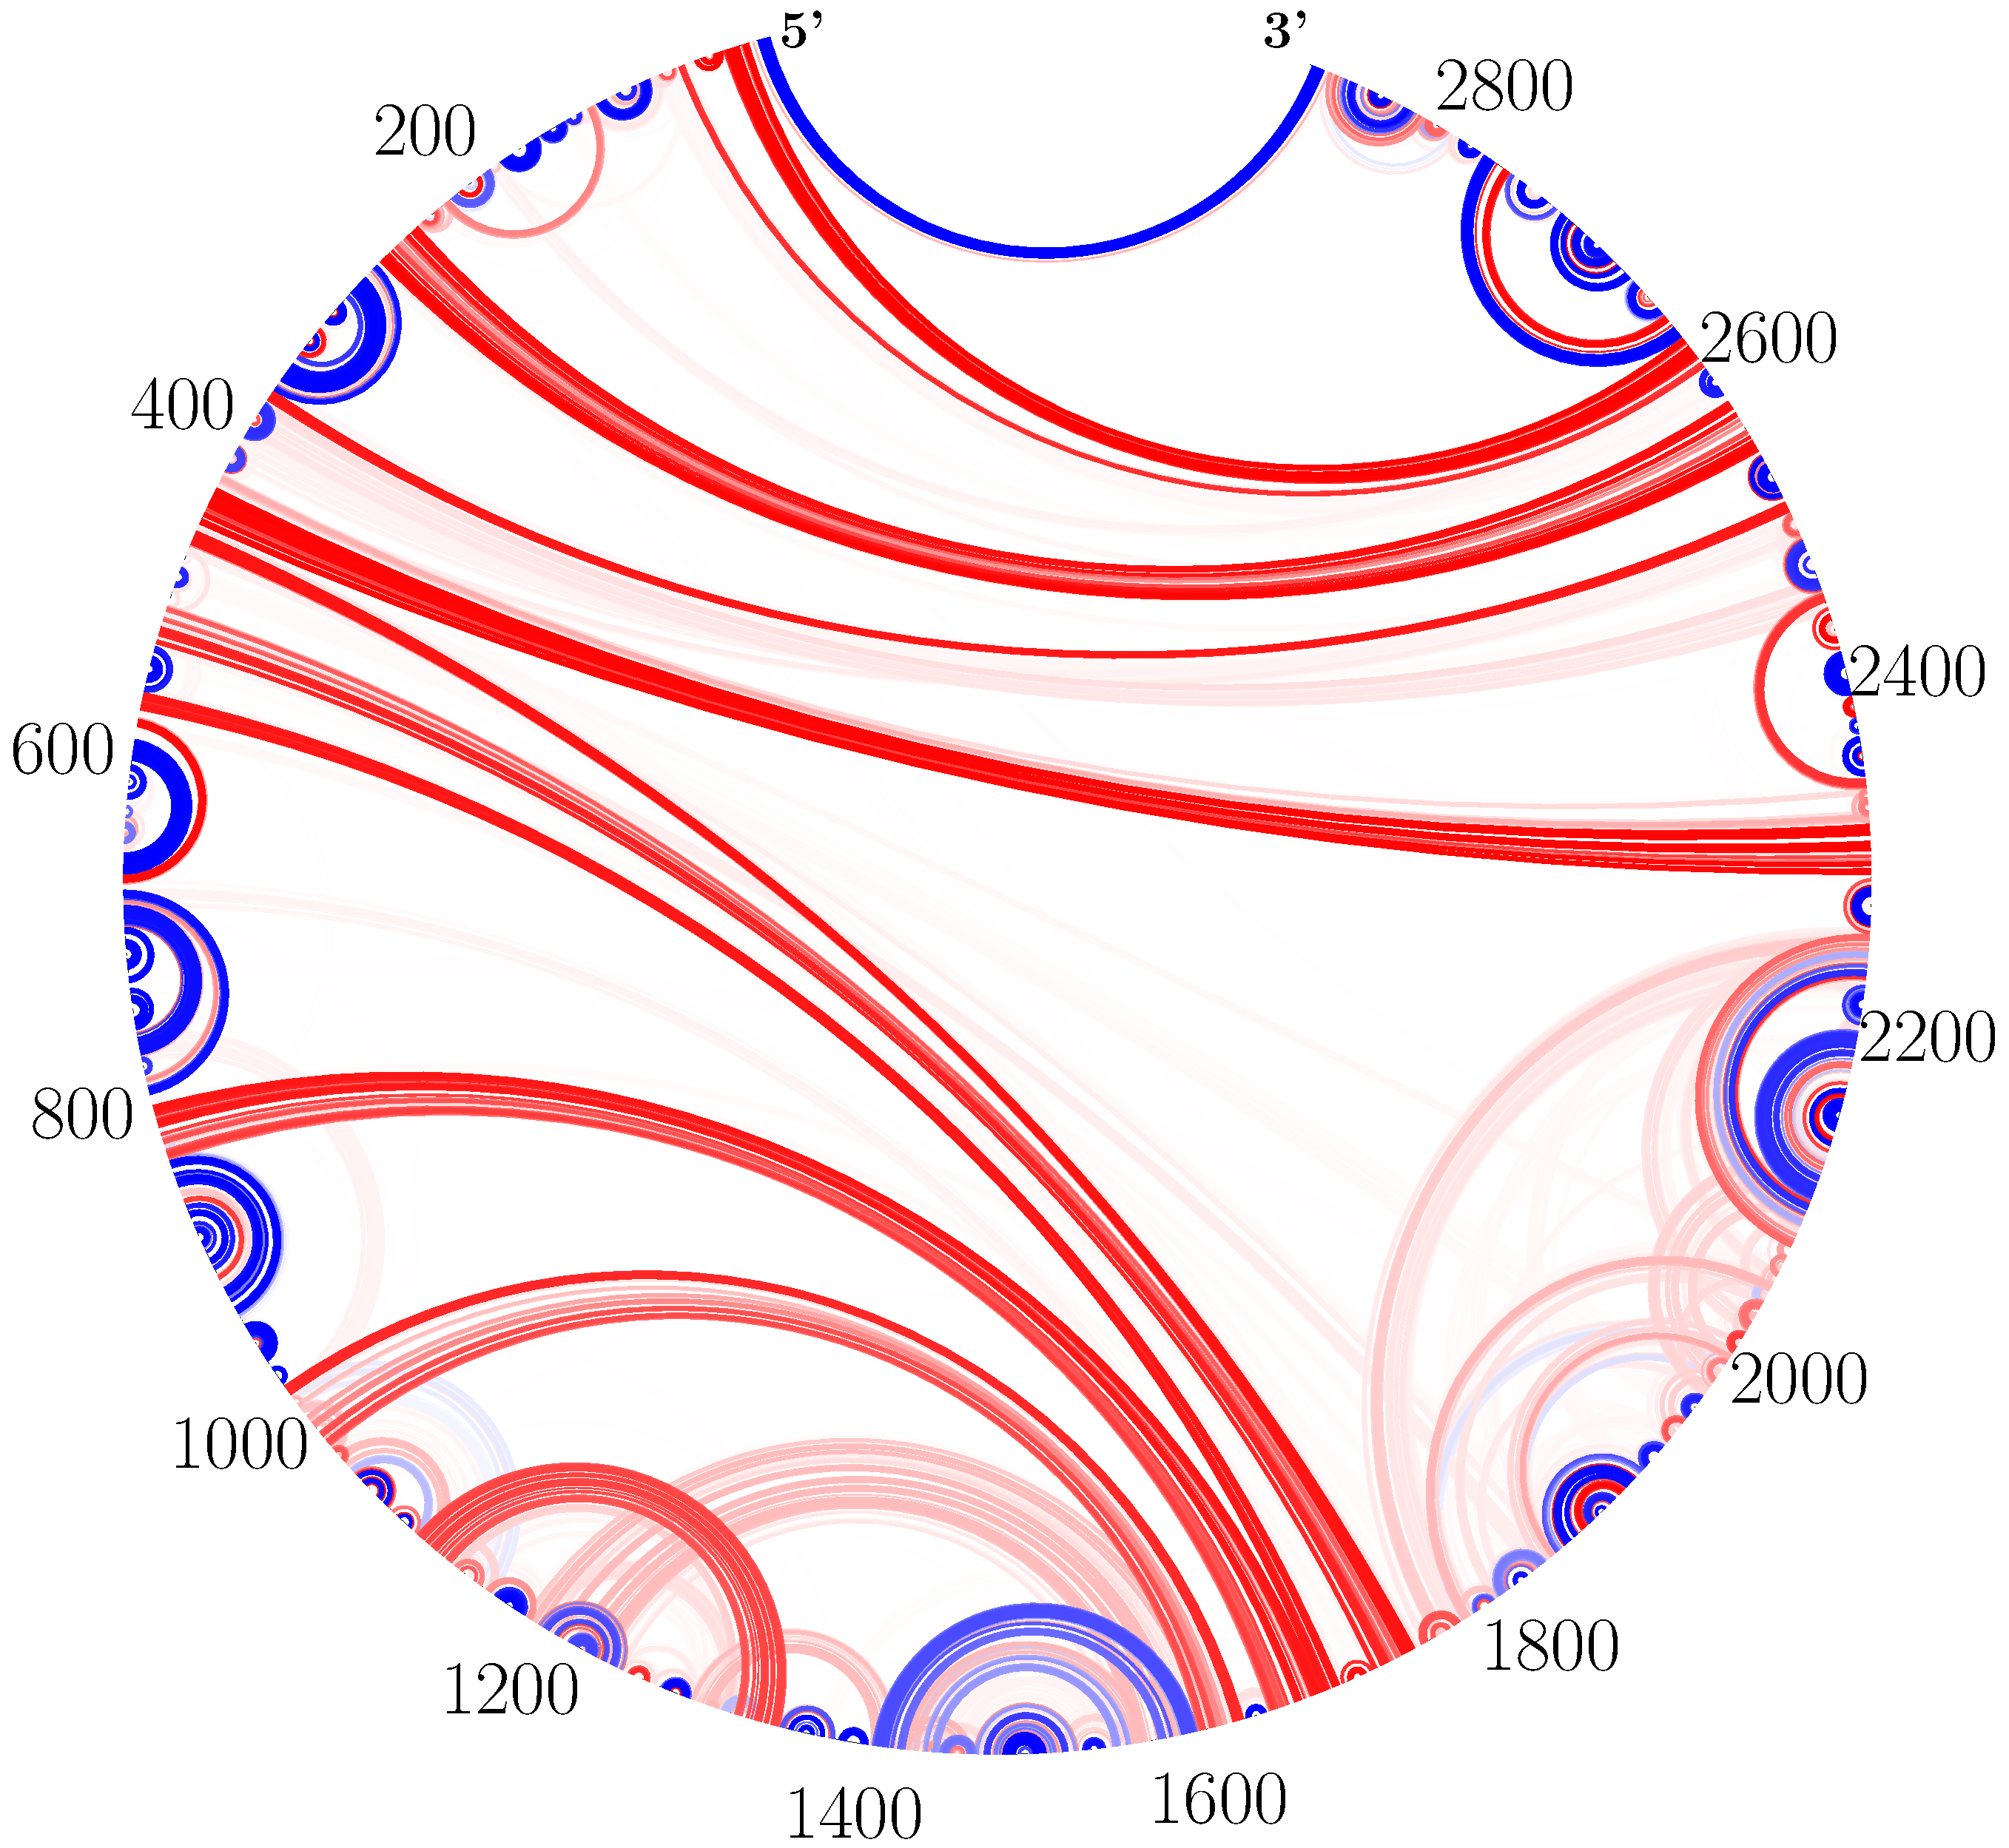
\includegraphics[width=0.22\textwidth]{figs/23s_vienna_example} &
\hspace{-0.35cm}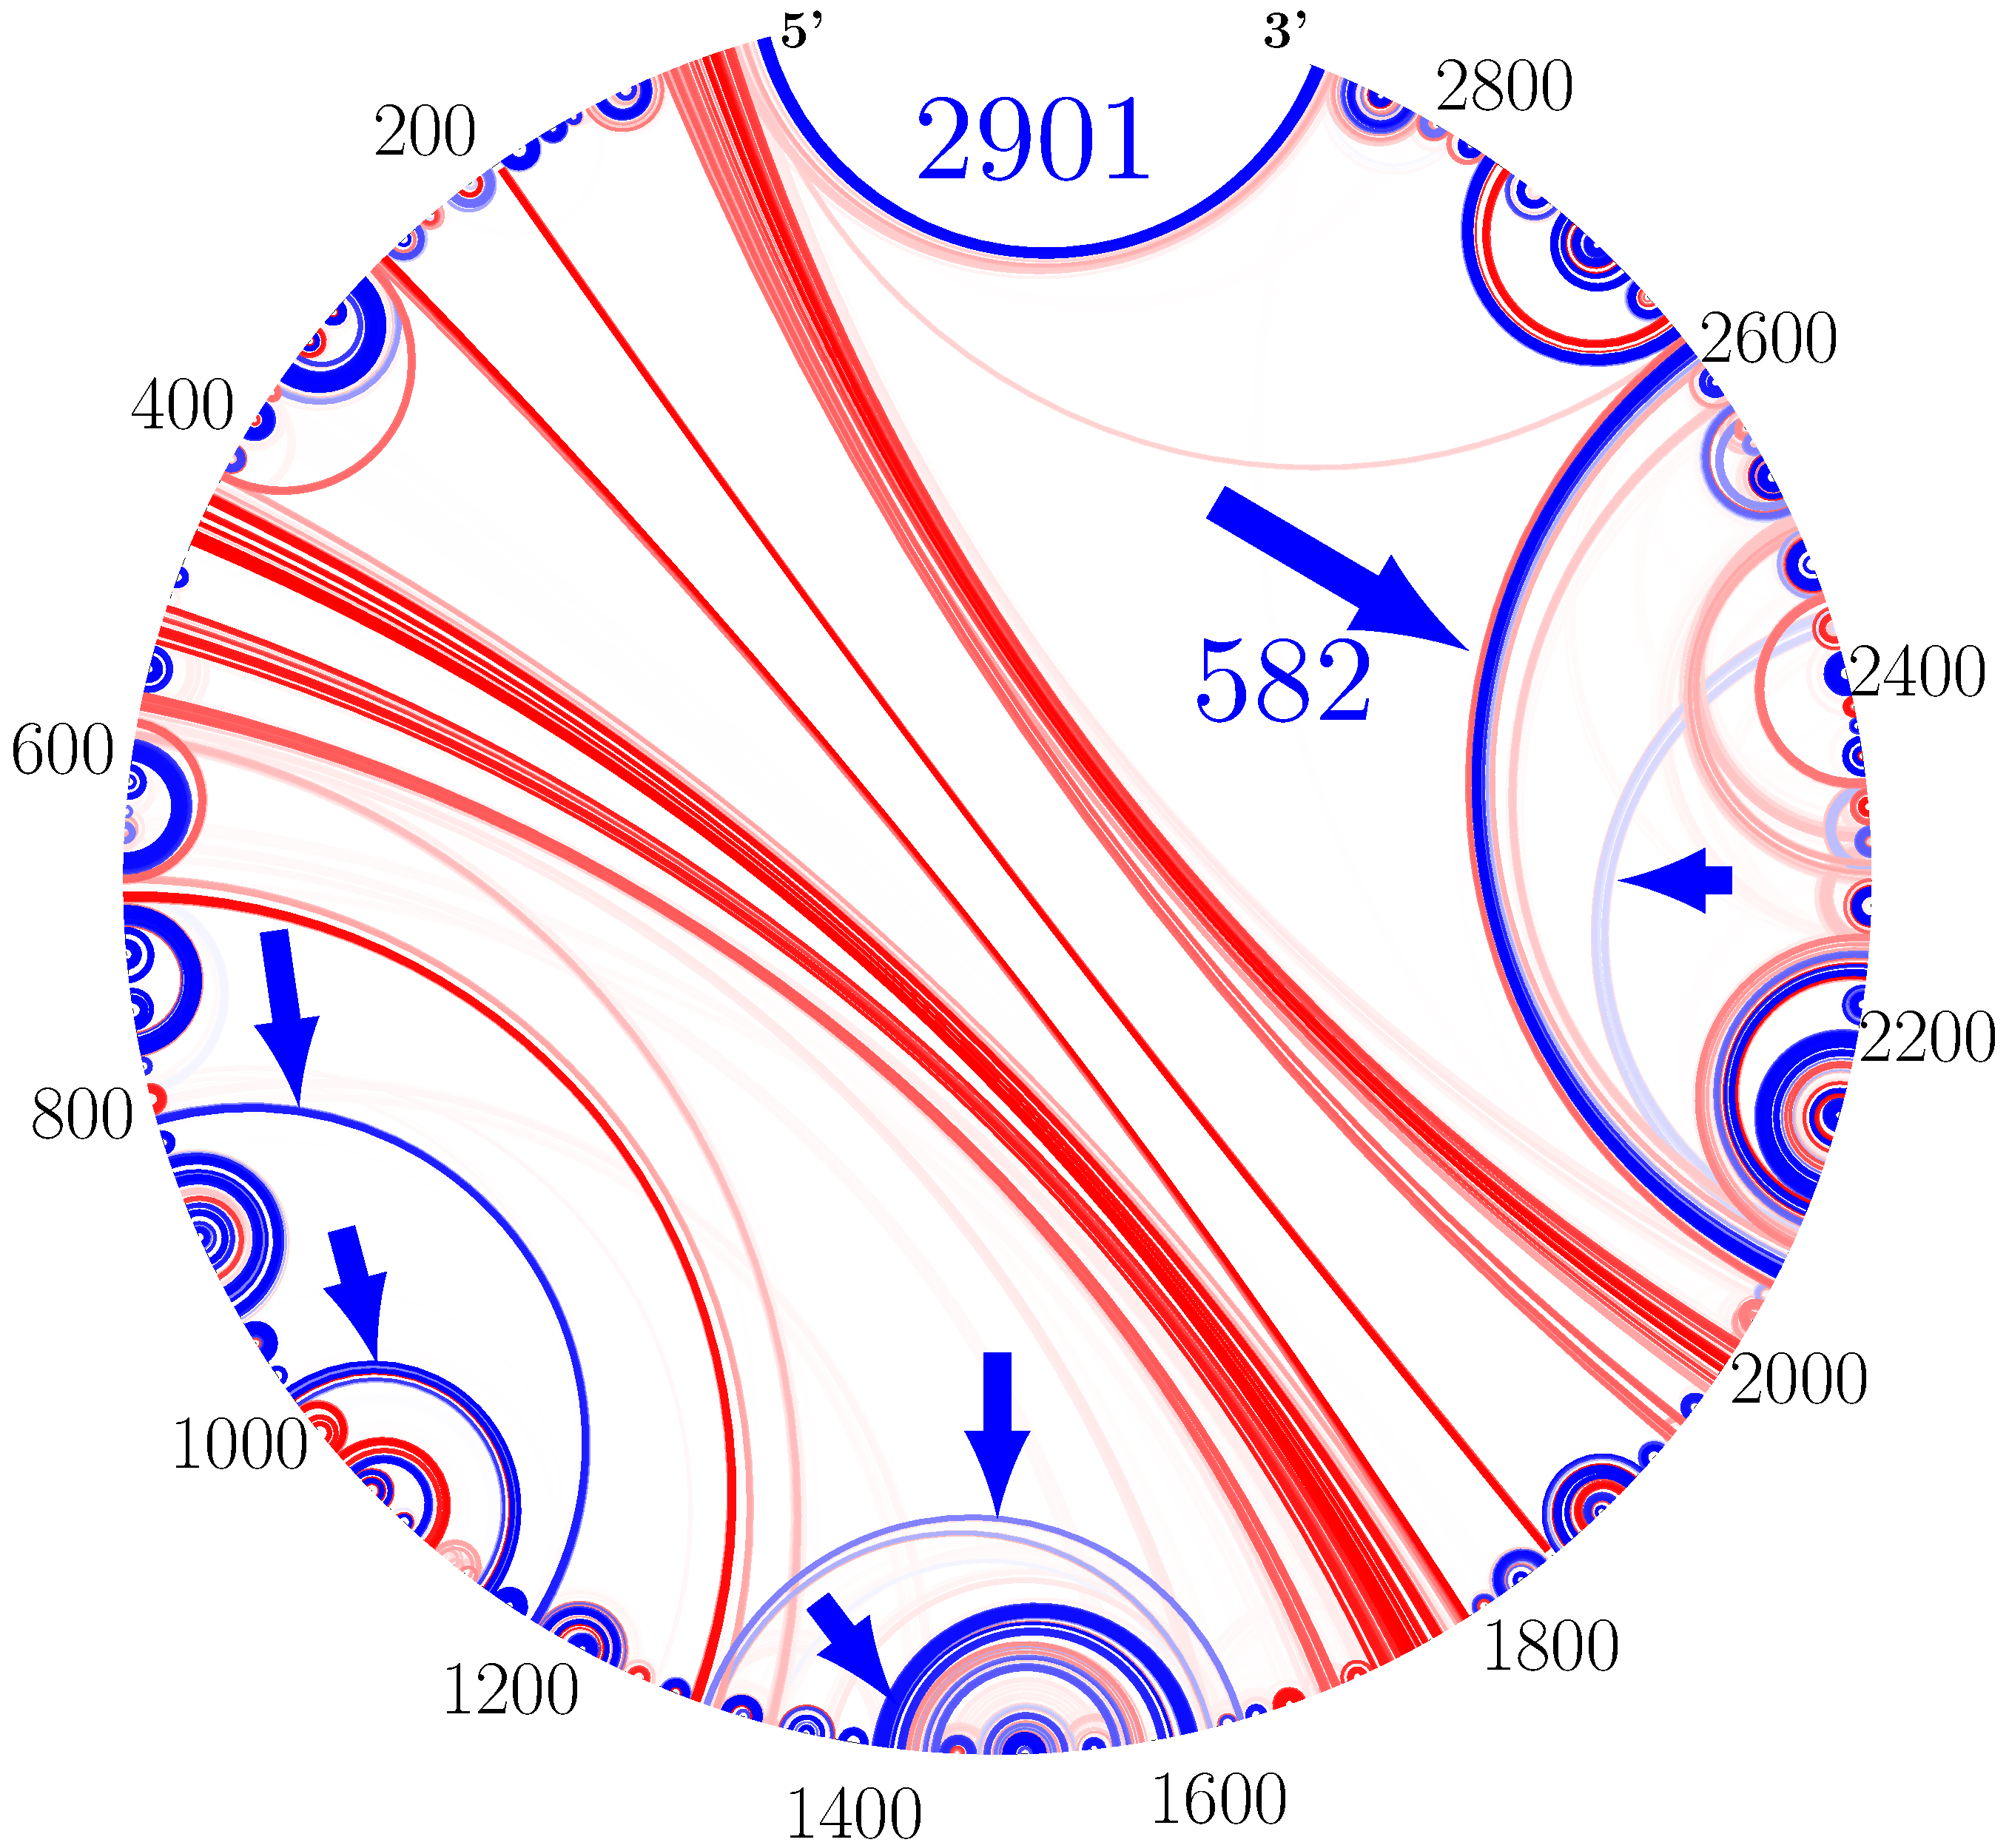
\includegraphics[width=0.22\textwidth]{figs/23s_example.pdf} \\
&\hspace{-4.cm} \panel{G} & \hspace{-4.6cm}\panel{H} & \hspace{-4.6cm}\panel{I} & \hspace{-4.6cm}\panel{J}\\[-0.4cm]
\raisebox{.4cm}{\rotatebox{90}{{\it C.~ellipsoidea} Group I Intron}}&
\hspace{-0.2cm}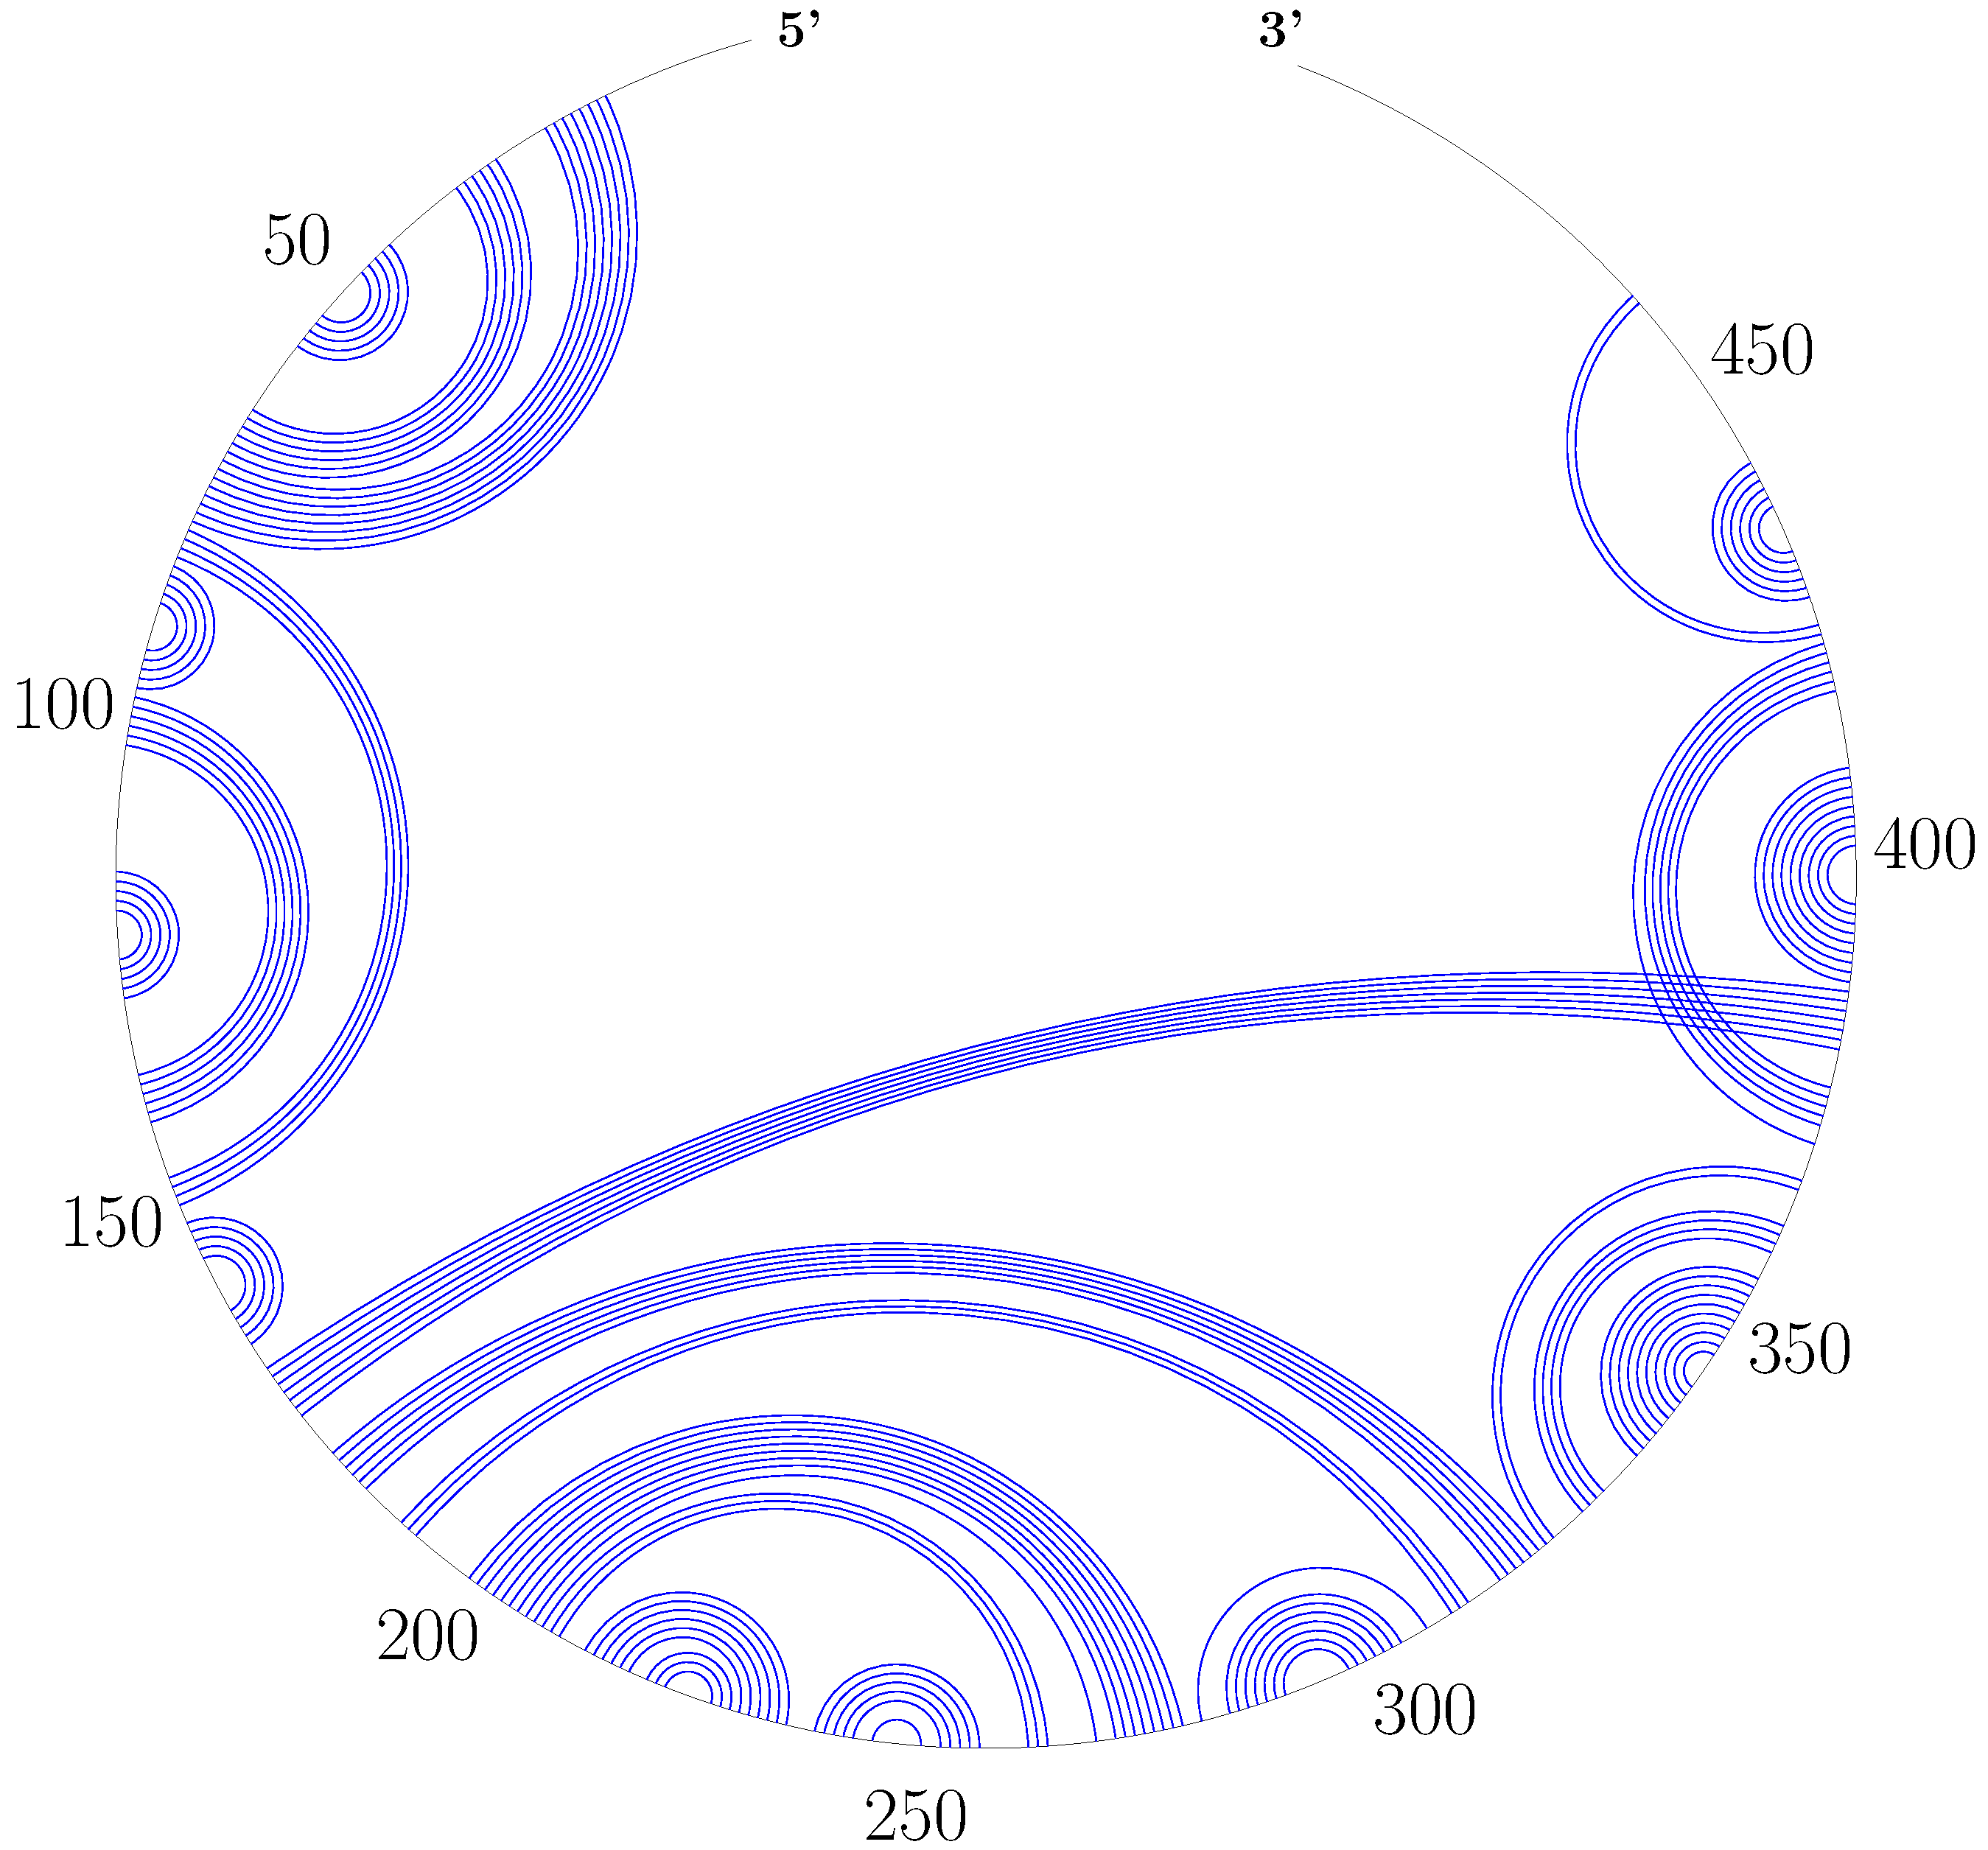
\includegraphics[width=0.22\textwidth]{figs/grp1_gold} &
\hspace{-0.35cm}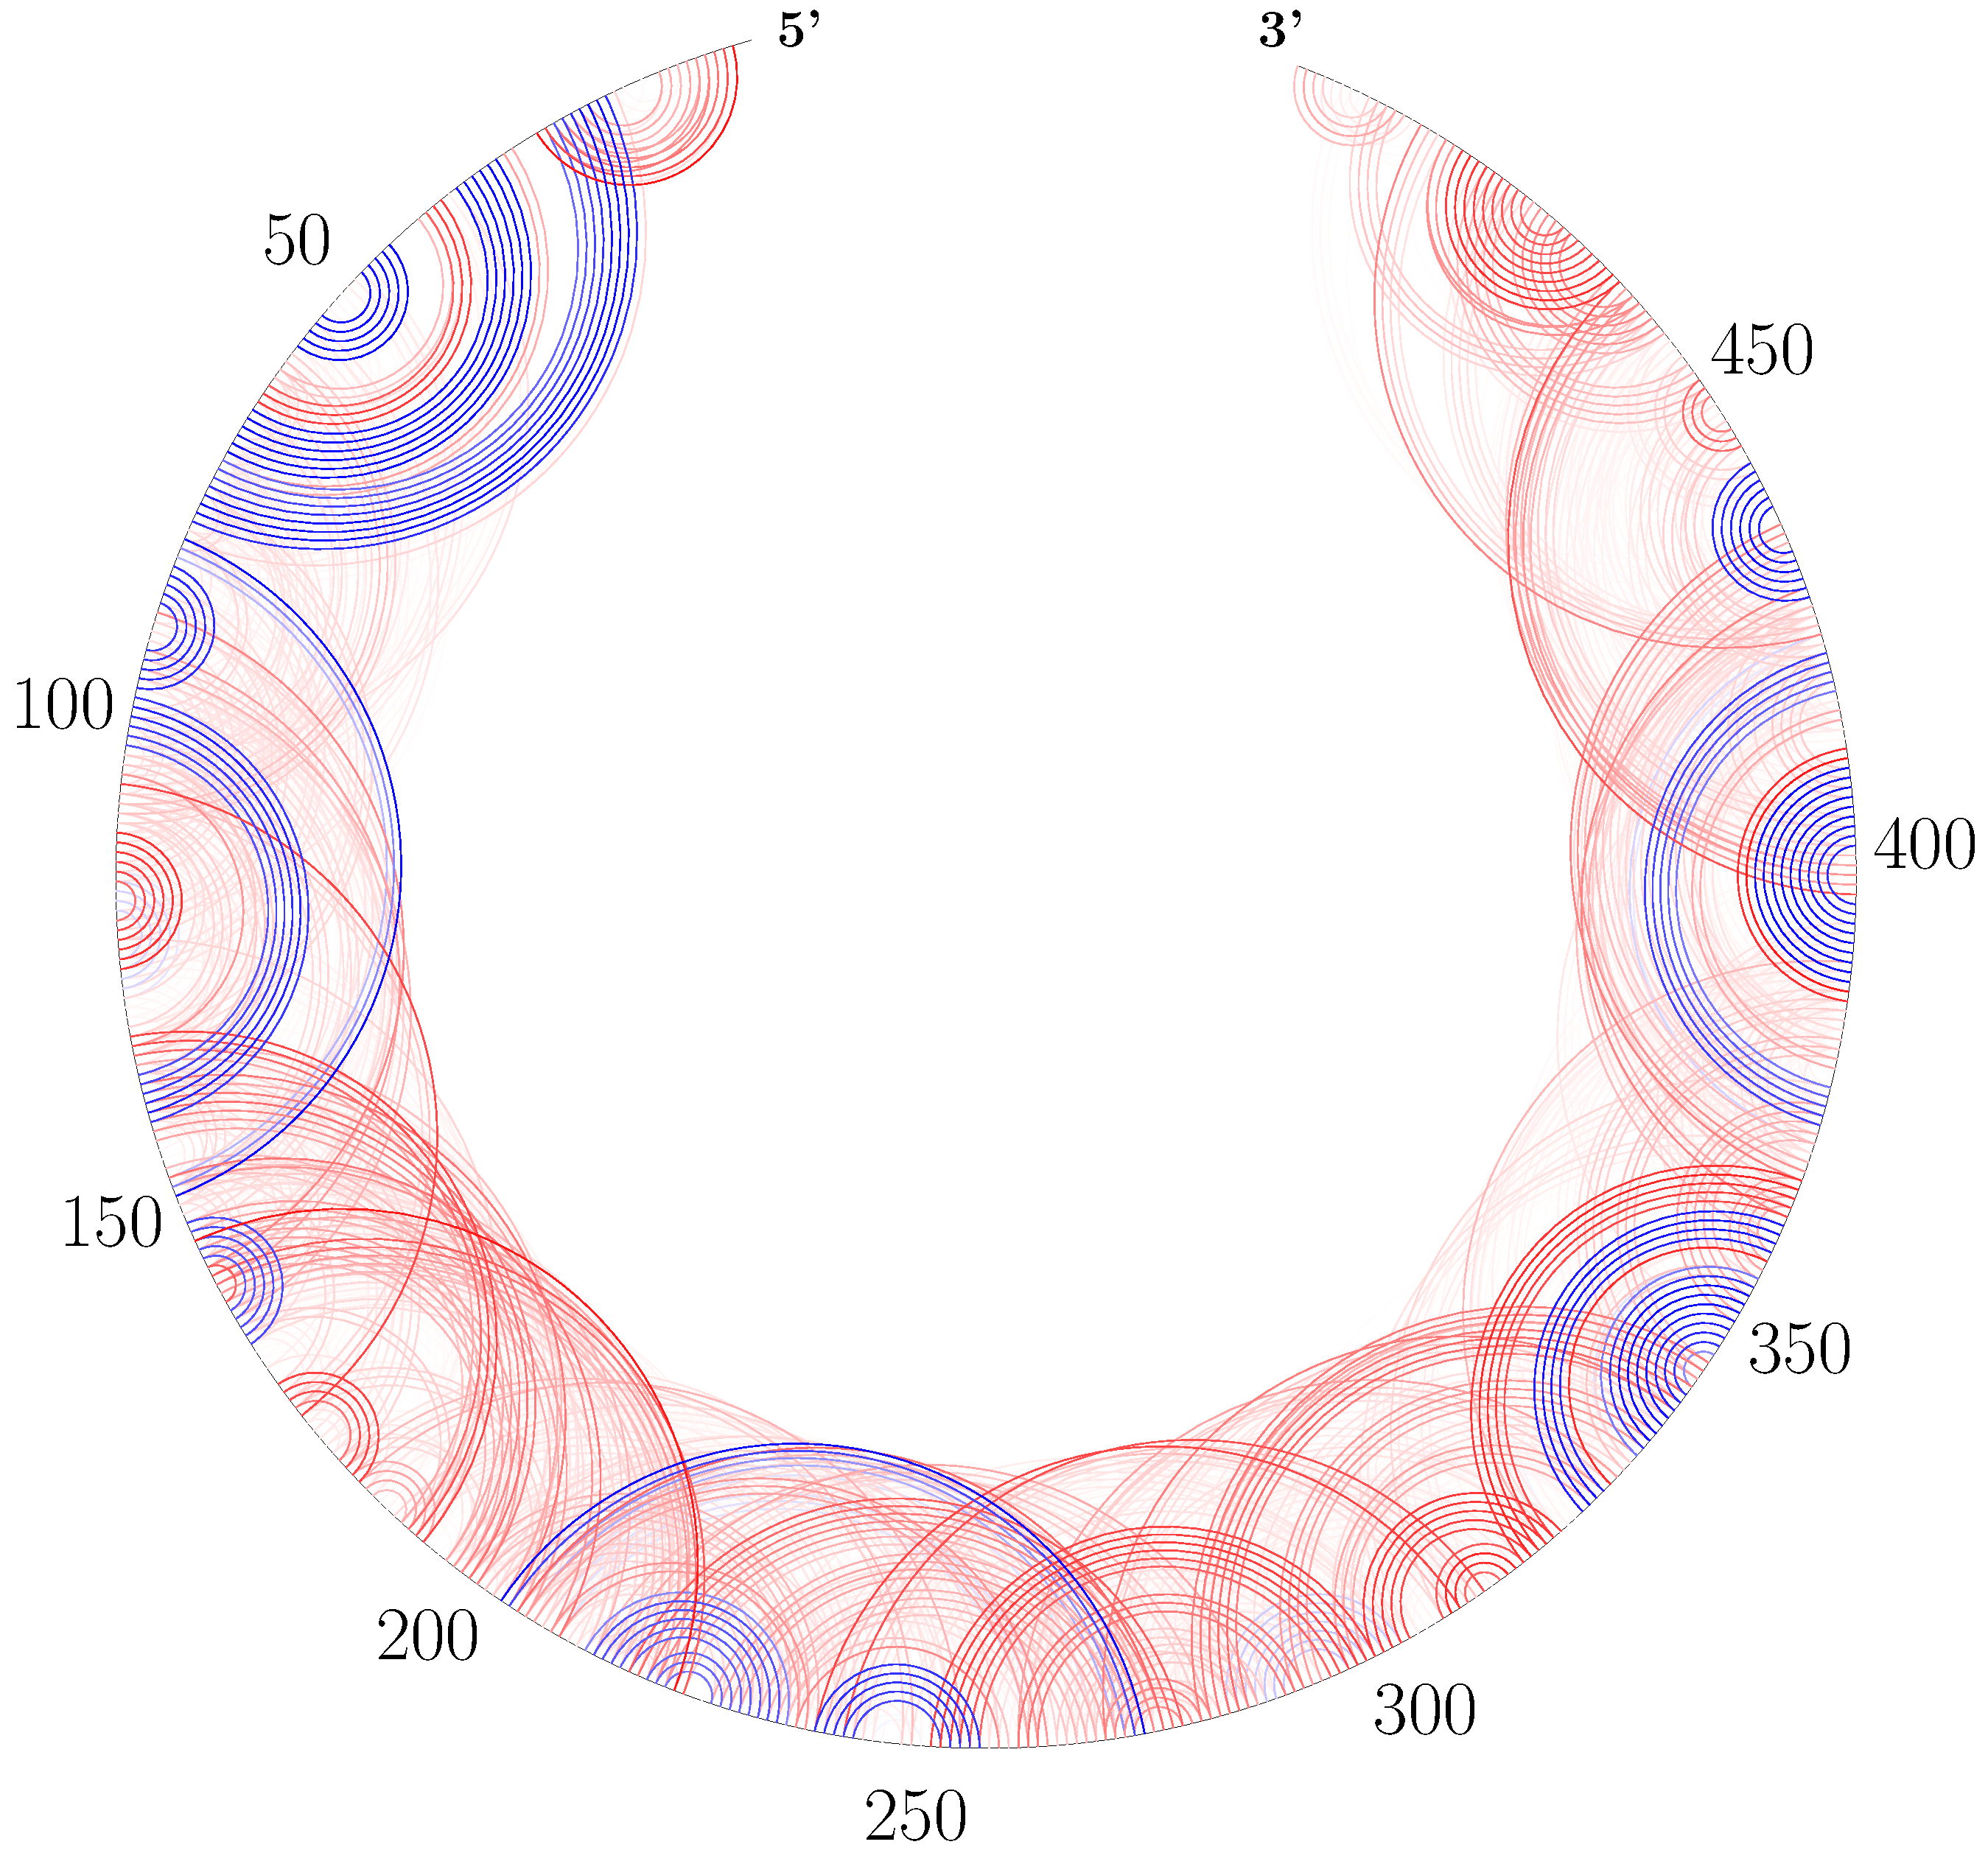
\includegraphics[width=0.22\textwidth]{figs/grp1_vienna_plfold_example.pdf} &
\hspace{-0.35cm}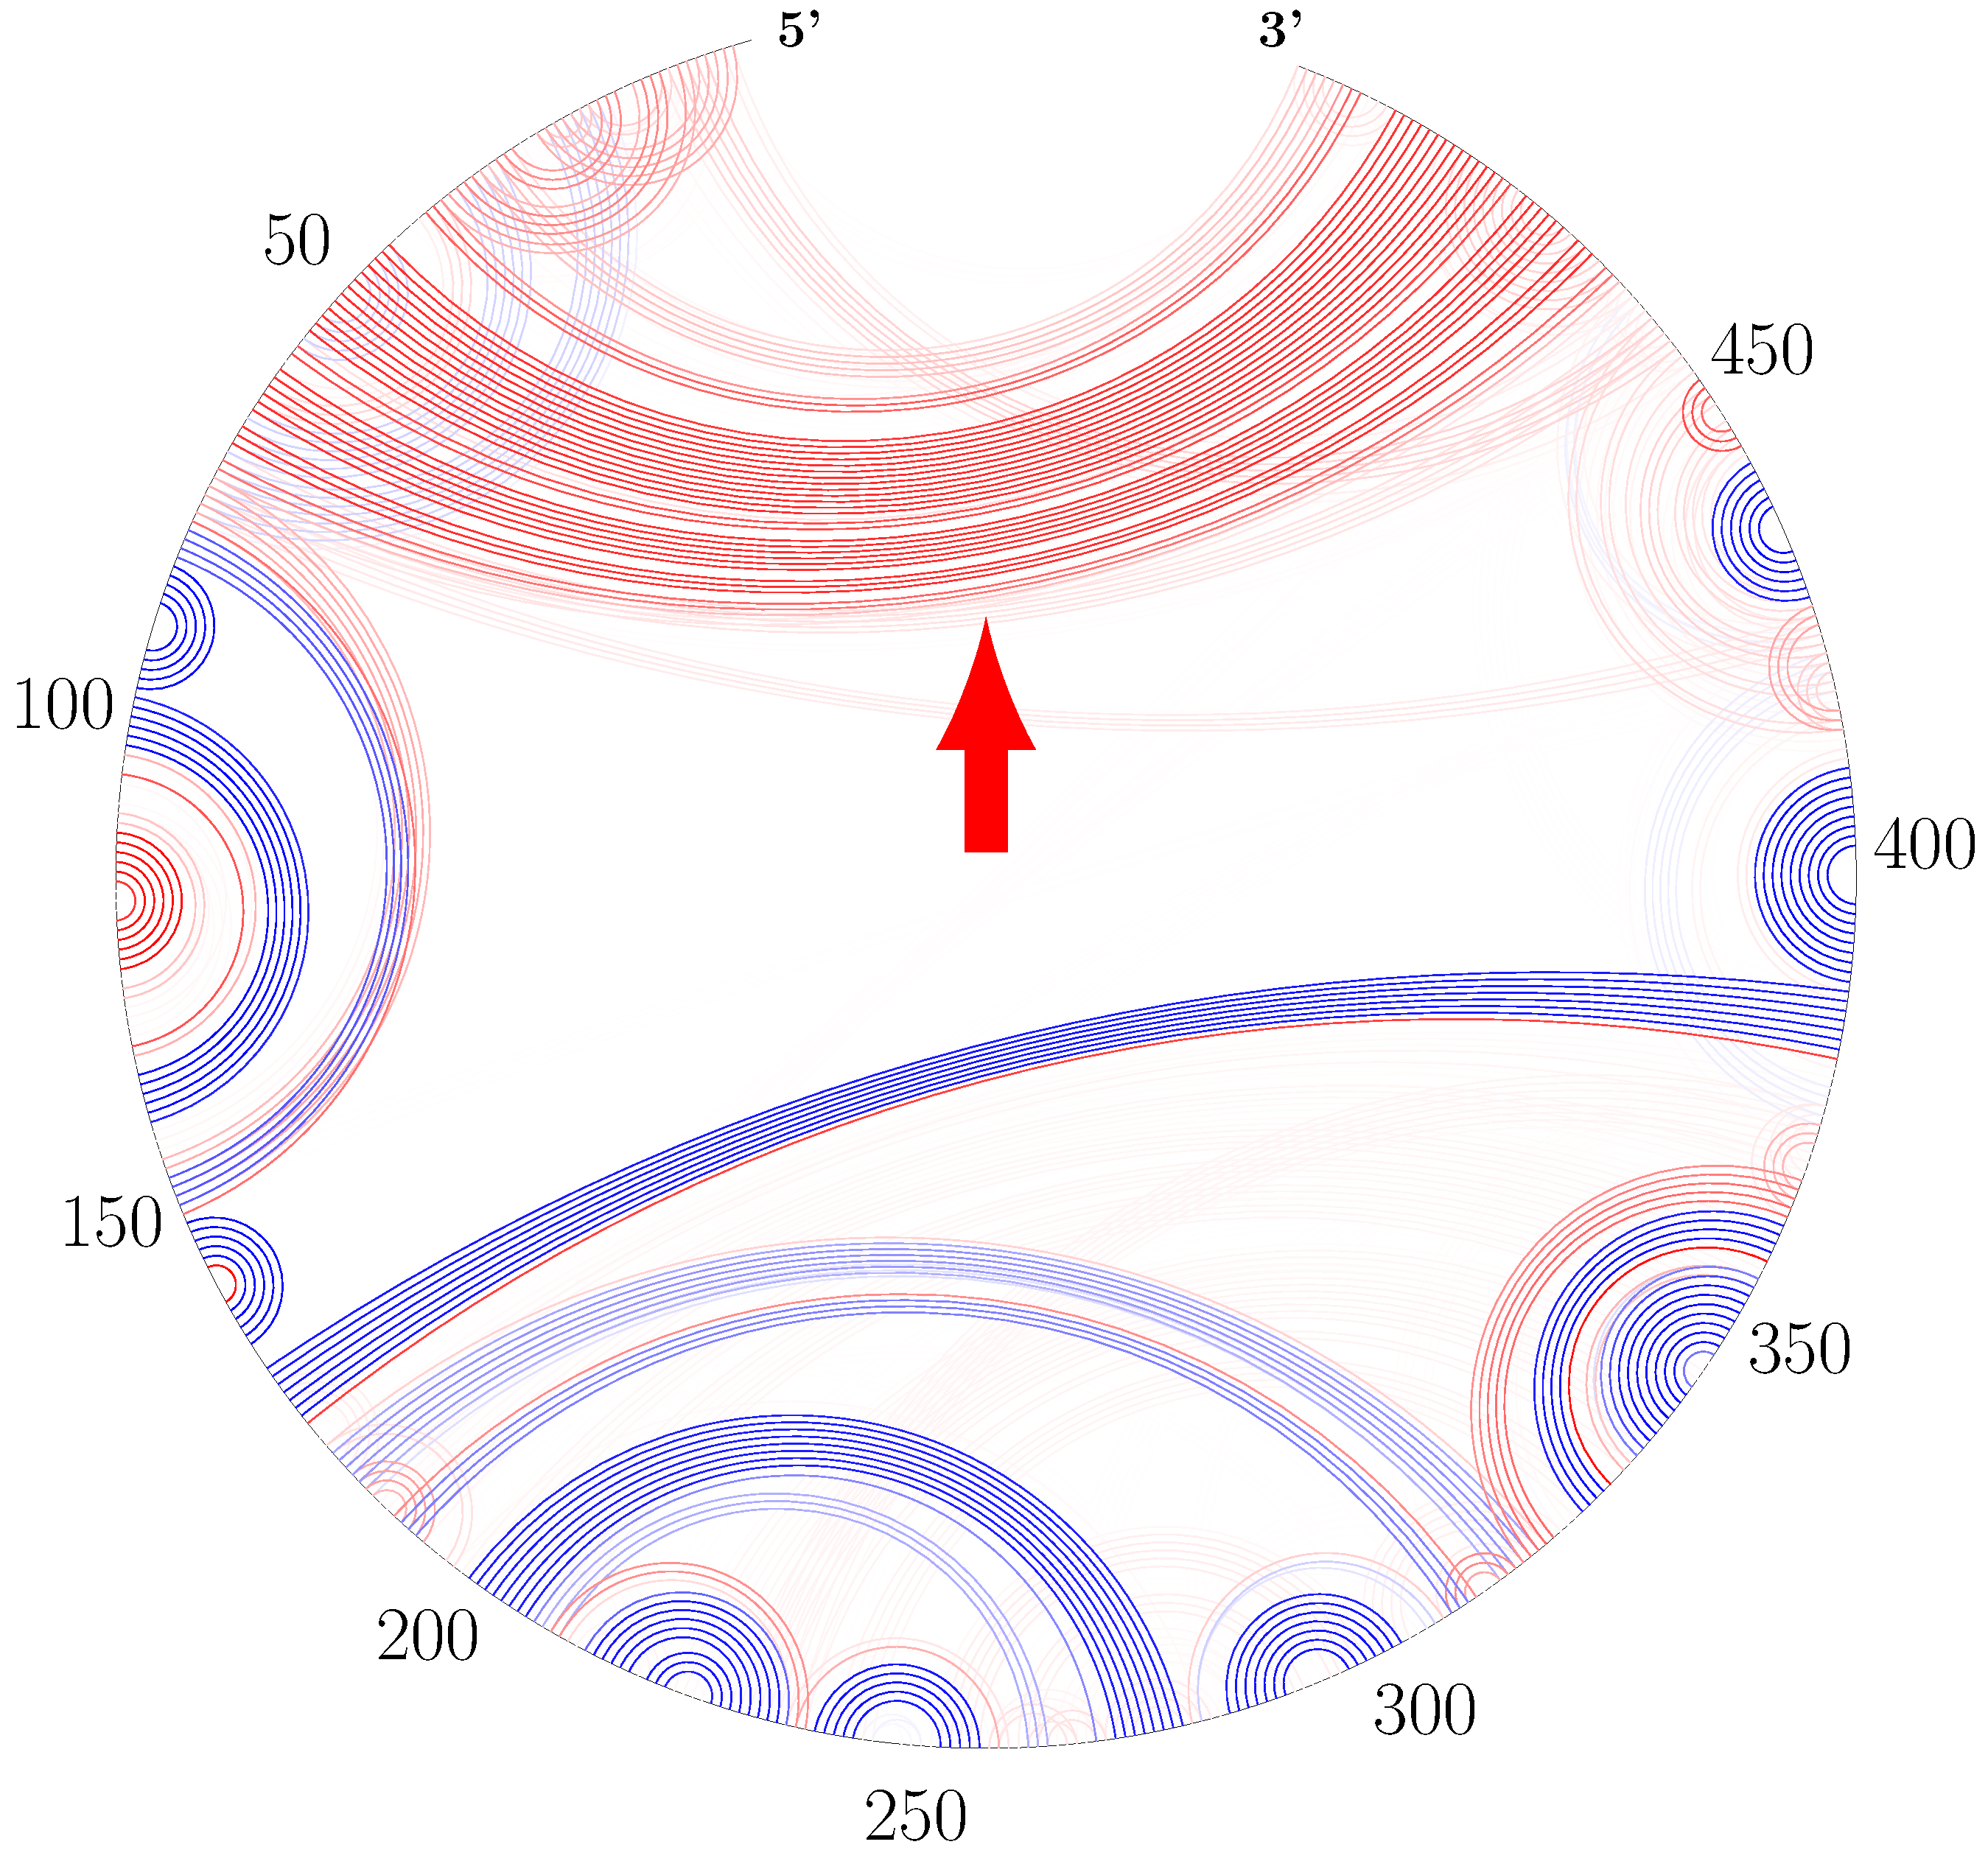
\includegraphics[width=0.22\textwidth]{figs/grp1_vienna_example} &
\hspace{-0.35cm}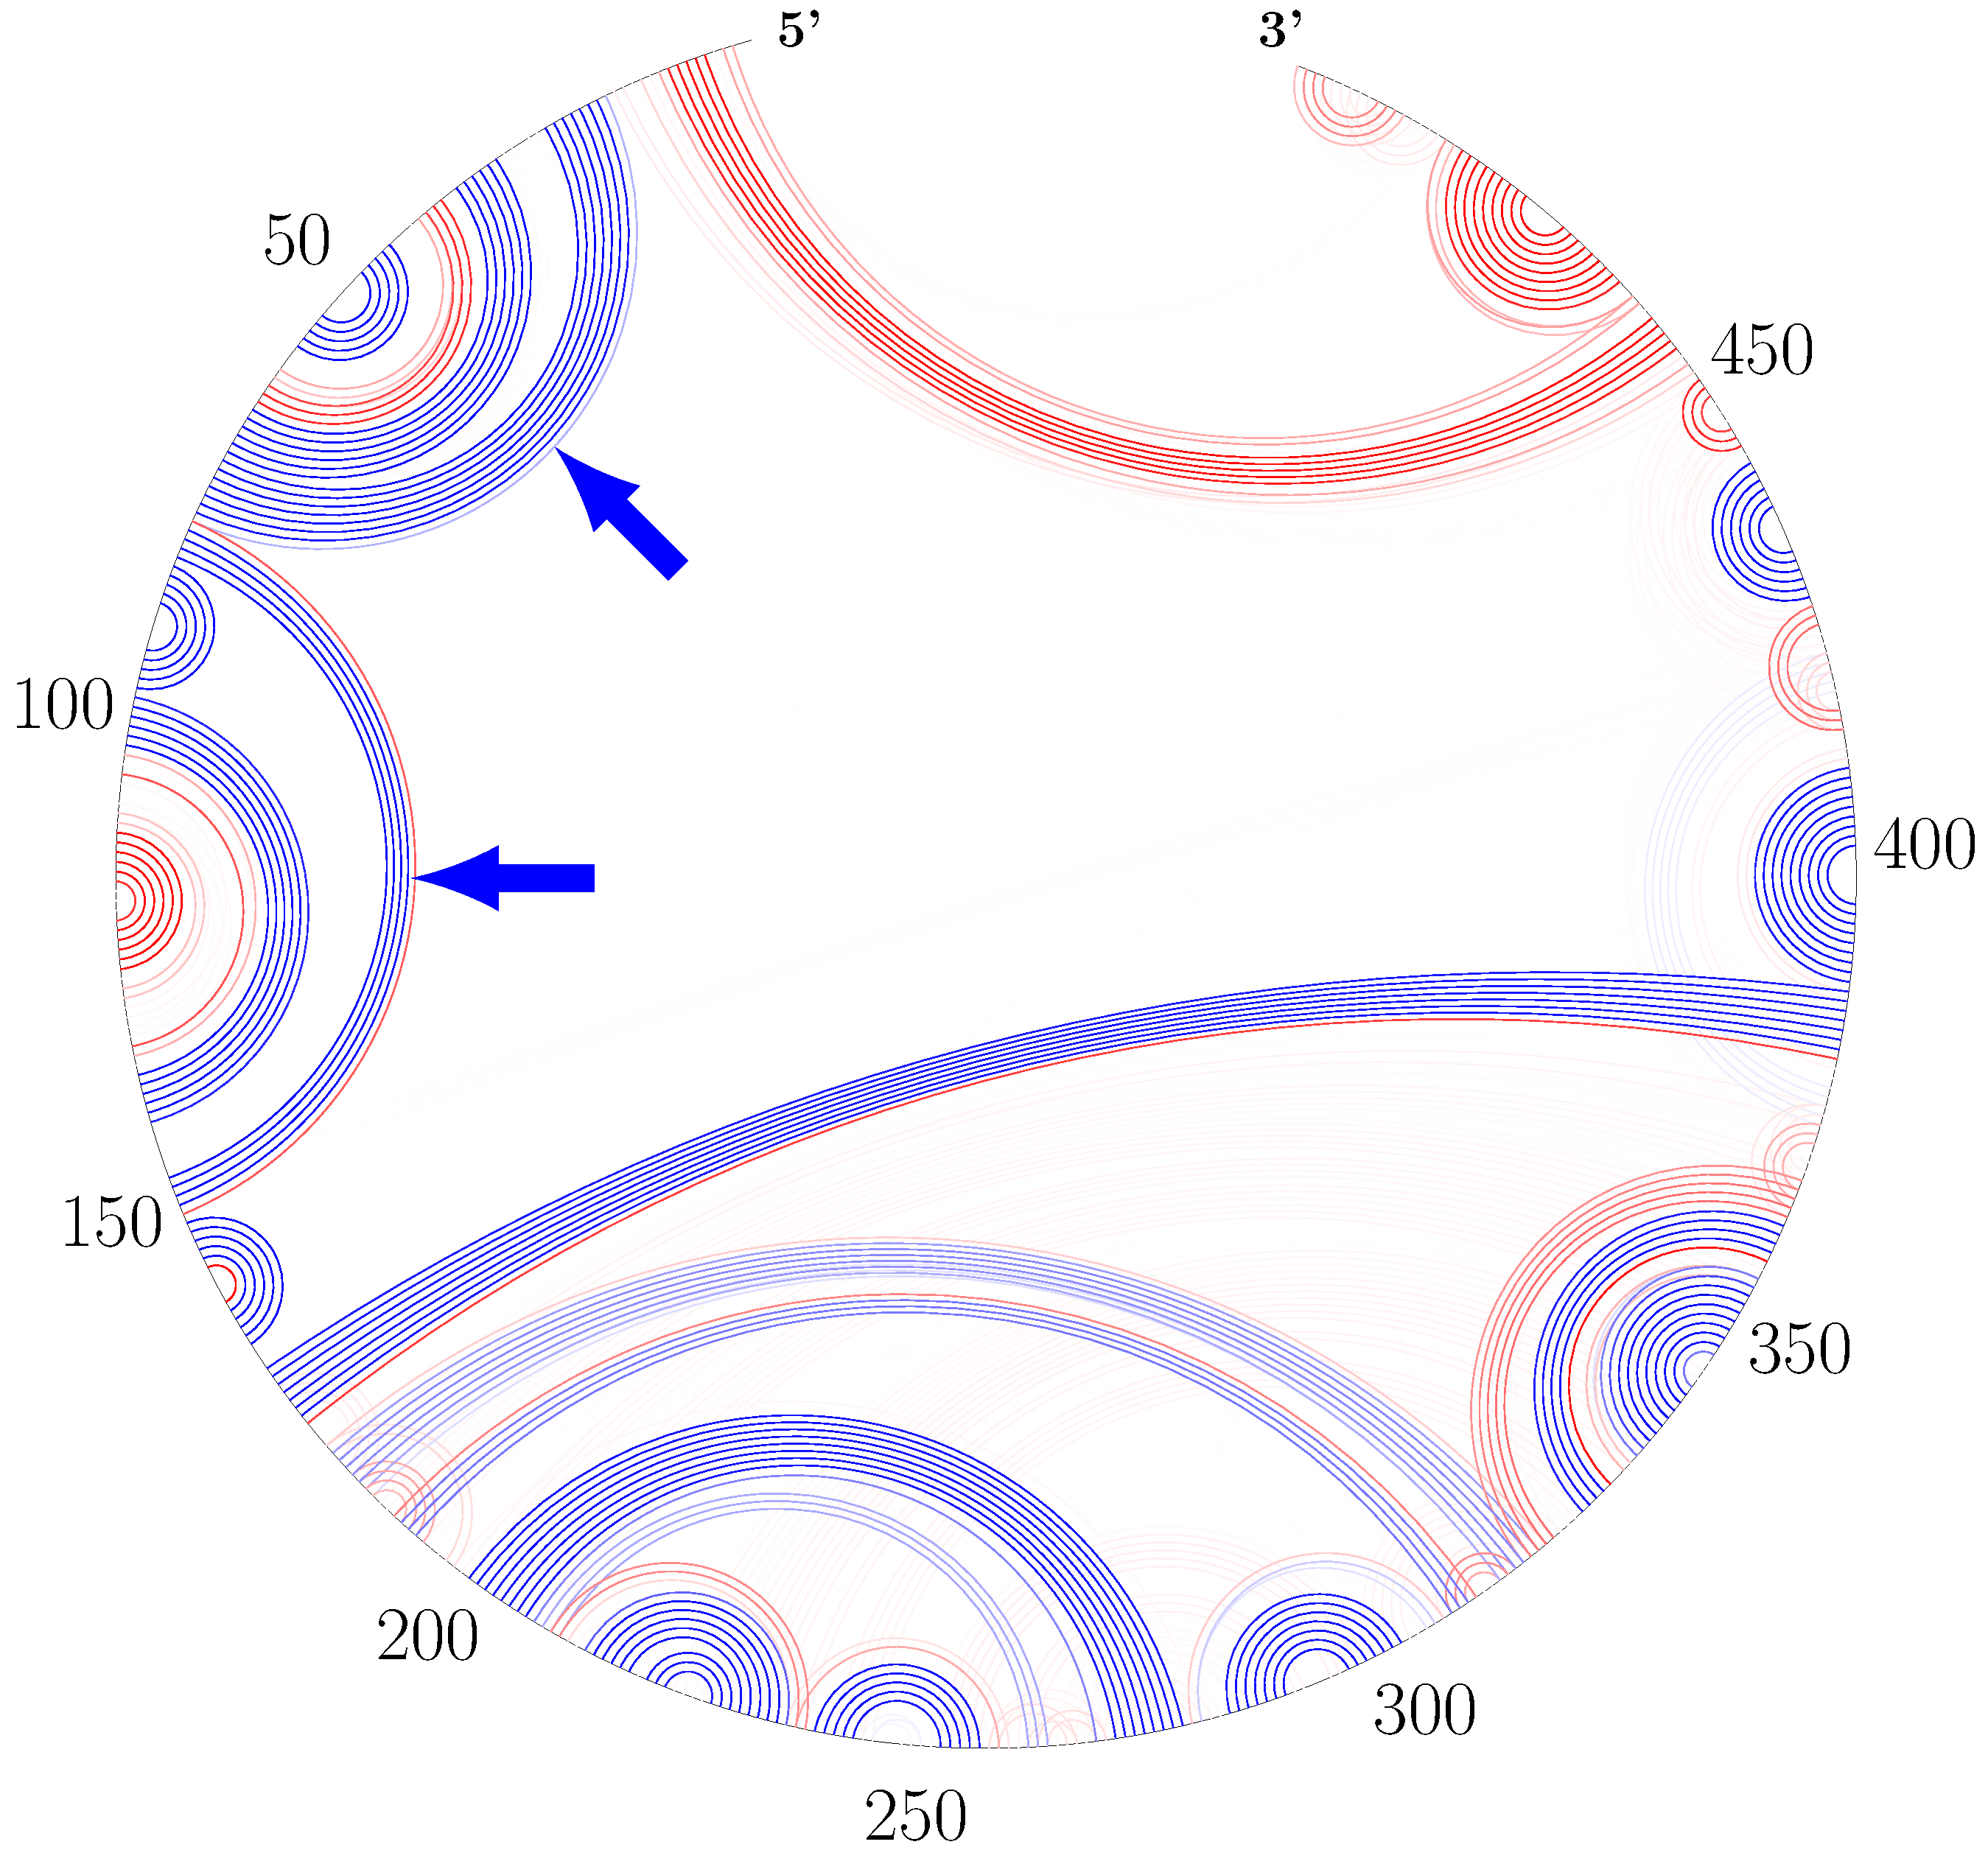
\includegraphics[width=0.22\textwidth]{figs/grp1_lpv_example.pdf}
\\[-0.2cm]
\end{tabular}
\caption{{\bf A}: Ensemble defect (expected number of incorrectly predicted nucleotides; lower is better) comparison between \viennarnafold and \linearpartition on the ArchiveII dataset.
  {\bf B}: Ensemble defect difference for each family.
  \linearpartition has lower ensemble defects for longer families:
   on average 56.3 less incorrectly predicted nucleotides on 23S rRNA and 8.3 less over all families.
  {\bf C--F}: An example of \ecoli 23S rRNA (shaded point in {\bf A}). 
  {\bf C}: Circular plot of the ground truth.
{\bf D--F}: Base pair probabilities from \viennarnaplfold (with default window size $70$), \rnafold and \linearpartition, respectively; 
Blue denotes pairs in the known structure and Red denotes predicted pairs not in the known structure.  
  The darkness of the line indicates pairing probability.
%  with the darkest lines close to a probability of 1. 
  {\bf G--J}: Circular plots of {\it C.~ellipsoidea} Group I Intron. 
%base pairs in the ground truth are in blue;
% blue and red indicate correct and incorrect base pairs,
% respectively, 
% and color darkness represents probabilities.
See Fig.~\ref{fig:example} 
% and~\ref{fig:circular_grp1} 
for another view of this example. % {\it C.~ellipsoidea} Group I Intron.
\label{fig:ensemble}
\vspace{-0.2cm}
}
\end{figure*}
